
\newcounter{Tcounter}
\newcommand{\sorSzam}{\stepcounter{Tcounter}\theTcounter}

\section{Termékek keresése a tudásbázisban szereplő technológiákhoz kapcsolódóan}
\subsection{Termékek keresése}
A \textit{Segítség, építkezem!} weboldal a szakemberek keresése mellett lehetőséget biztosít az építkezésekhez szükséges termékek közötti böngészésre is, amihez egy külön felület tartozik (\kovAzon{T\_\sorSzam}). \\
A weboldalon a termékek kategóriái és alkategóriái munkafázisok, anyagok és szerszámok köré szerveződnek (\kovAzon{T\_\sorSzam}), például:
\begin{enumerate}
    \item Falazás
        \begin{itemize}
            \item Beton
            \item Tégla
            \item Vakolat
            \item Habarcskiegészítők
        \end{itemize}
    \item Tetőszerkezet
        \begin{itemize}
            \item Cserép
            \item Tetőfólia
            \item Szellőző és kiegészítők
            \item Hőszigetelés
        \end{itemize}
\end{enumerate}

A oldal rendelkezik egy belső adatbázissal, amiben a termékeket tárolja (\kovAzon{T\_\sorSzam}). A gyűjteményben való böngészés során a szakemberek kereséséhez hasonlóan lehetőség van előre meghatározott szűrőket használni, illetve szabad szavas kereső is rendelkezésre áll (\kovAzon{T\_\sorSzam}). \\
A szűrők a termékek adatai alapján a következők lehetnek:
\begin{itemize}
    \item termék neve,
    \item termék főkategóriája,
    \item termék alkategória a főkategórián belül,
    \item paraméterek (a termék kategóriájától függően),
    \item ár,
    \item elérhetőség.
\end{itemize}
A keresési találatokat lehetőség van rendezni is (\kovAzon{T\_\sorSzam}). A rendezési szempontok a termékek kategóriájának megfelelően változnak, például falazásnál teherbíró képesség, szállítási idő.

\begin{figure}[h]
	\centering
	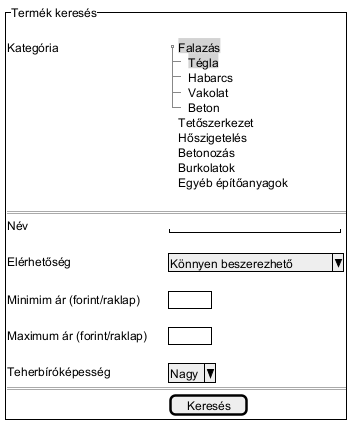
\includegraphics[scale=0.5]{img/termek_keres.png}
	\caption*{Termék keresése}
	\label{fig:term_ker}
\end{figure}

\begin{figure}[h]
	\centering
	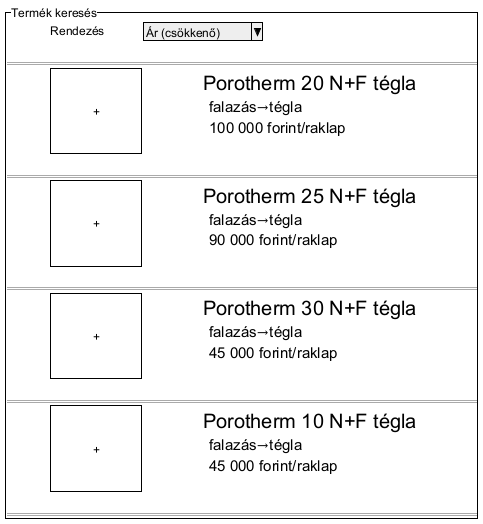
\includegraphics[scale=0.4]{img/termek_eredmeny.png}
	\caption*{Termék keresési eredménye}
	\label{fig:term_ker_ered}
\end{figure}

\clearpage
\subsection{Termékek bővítése, módosítása}
A weboldal belső adatbázisa a szakemberek javaslatai alapján kerül kialakításra, bővítésre (\kovAzon{T\_\sorSzam}). A szakembereknek lehetőségük van előterjeszteni egy terméket a megfelelő adatokkal, ami majd az adminisztrátorok által kerül jóváhagyásra vagy elutasításra. \\
Az új termékek esetén a következő adatokat kell megadni (\kovAzon{T\_\sorSzam}):
\begin{itemize}
    \item név,
    \item főkategória,
    \item alkategória a főkategórián belül,
    \item kategóriának megfelelő paraméterek,
    \item rövid leírás,
    \item fotó.
\end{itemize}

 Az adatbázisban szereplő termékeket a tudásbázisban szereplő technológiák\-hoz kell rendelni (\kovAzon{T\_\sorSzam}).

Az adatbázisban már szereplő termékek szintén szakemberek javaslatára, adminisztrátori jóváhagyással módosíthatóak (\kovAzon{T\_\sorSzam}). A változások követhetőségének érdekében a termékek verziószámokkal vannak ellátva (\kovAzon{T\_\sorSzam}). Módosítások után, az egyes verziókhoz kötve megjelenítésre kerül, hogy pontosan mi és miért változott. Szerkesztés indoka lehet például új verzió elérhetősége a piacon, vagy korábbi hibás adatbevitel korrigálása.


Egy termék módosításról az érintettek értesítést kapnak (\kovAzon{T\_\sorSzam}). Érintettnek számí\-tanak a következő felhasználók:
\begin{itemize}
    \item bárki, akinek az építkezésében felmerült az adott termék (például a tervezési fázisban elmentette a korábbi a változatot),
    \item kivitelezők, akik az adott terméket szokták használni.
\end{itemize}


\subsection{Szakemberek kapcsolata a termékekkel}
A szakembereknek lehetőségük van magukhoz rendelni azokat az adatbázisban szereplő termékeket (\kovAzon{T\_\sorSzam}), amelyekkel van tapasztalatuk. A termékek oldalán megjelenítésre kerül, hogy mely mesteremberek dolgoztak már ezzel, illetve a szakemberek profilján is megtekinthető, hogy milyen termékekkel van gyakorlatuk (\kovAzon{T\_\sorSzam}).

\subsection{Külső kapcsolatok}
A belső adatbázis mellett az oldal lehetőséget biztosít külső adatbázissal való összeköttetés létesítésére is (\kovAzon{T\_\sorSzam}). Lehet például partnerségi kapcsolatot kialakítani építőanyag kereskedőkkel, beszállítókkal. Kapcsolatok kialakítására a szakemberek tehetnek javaslatot, de a tényleges megvalósításhoz kell jóváhagyás, moderálás az üzemeltetőtől (\kovAzon{T\_\sorSzam}).


A külső adatbázisokból a termékek importálásra kerülnek, és kereshetőek lesznek az oldal felhasználói számára (\kovAzon{T\_\sorSzam}).
